
\chapter{序論}\label{chap:intro}

%\section{スピントロニクスとスピン流物理}


%電子とは負の電荷を持ち,固体物理の様々な特性を支配する基本粒子である.この電荷という内部自由度に加え,電子は角運動量という内部自由度も持つ.この角運動量は古典的に見れば電子がスピンしていることに対応しており,スピンと呼ばれる.このスピンは電子の相対論的量子力学におけるDirac方程式より導かれ,また磁性の起源ともなっている.

%従来のエレクトロニクスは電子における電荷の自由度のみに注目して発展を遂げた.しかし,電子にはスピンという.

身の回りを見回してみると家電製品や通信機器など多くのものがエレクトロニクスによって生み出されたものだと気づく.今の世界でエレクトロニクスはなくてはならない技術となっている.しかしエレクトロニクスは電子の電荷を利用することで展開している分野であり電子の持つもう一つの自由度,スピンを無視している.ここでスピンも電荷も利用しようとする学問がスピントロニクスである.スピンと電子の相互作用はナノスケールの長さで現れるため\cite{maekawa2002spin},1990年代におけるナノテクノロジーの大きな進歩がスピントロニクスの幕を上げたと言っても過言ではない.
スピントロニクスはスピンと電荷を組み合わせることによって革新的なデバイス機能を創り出そうとする分野である\cite{prinz1998magnetoelectronics,vzutic2004spintronics,wolf2001spintronics}.その発展は1988年における巨大磁気抵抗(GMR)の発見\cite{baibich1988giant,binasch1989enhanced}によって始まった.巨大磁気抵抗効果はGMR素子としてハードディスクドライブの磁気ヘッドなどに応用されていて,これは最初に成功したスピンデバイスとみなされている.
スピントロニクスの基本的な考え方は,今まで電子のスピンを無視して利用してきた電流に代わって,スピン分極した電子の流れであるスピン流を巧みに操るというものである.電荷に加えてスピンの自由度も考慮に入れると,今までは見えなかった電子の持つ効果や機能性が現れる.その一つが磁場を介さない磁化制御である.スピン流と磁化の相互作用はまだ解明されていない部分が大きいが,近年スピン流が磁化に与えるトルクの大きさを見積もる報告がされている\cite{hayashi2014quantitative,yang2014platinum}.本研究では,金属の界面に影響を与える自己組織化単分子膜(self assembled monolayer : SAM)という有機分子膜\cite{de2005tuning,love2005self,xu2014regulating}を用いて常磁性金属の表面状態を変化させ,そのときのスピン流によるトルクの変化を調べた.この研究によりスピン流によるトルクと金属表面との結びつきについて理解が深まるだけでなく,スピントロニクスの発展に寄与することが期待される.
本章ではまず磁化の運動方程式としてLandau-Lifshitz-Gilbert(LLG)方程式を導入する.そしてスピン流およびスピン蓄積を説明し,それらと磁化の相互作用として現れるスピン軌道トルクを定義する.

%\section{スピントロニクスと磁化制御}


%スピン流は,薄膜などの磁気構造に流すことで局所的な磁気電子と直接相互作用を引き起こせるため,磁化をコントロールする効果的な方法として注目を集めている.
%電気的に磁化をコントロールしている応用のひとつとして,商業的に利用されているSTT(spin transfer torque) MTJ(magnetic tunnel junction)メモリである.
%STTでは,磁化方向を固定された強磁性体層(固定層)に垂直に流れた電子はその磁化方向にスピン分極する.このスピン流は絶縁体を超えて,隣の強磁性体層にトルクを与え,磁化の方向を決めることができる.
%STTではスピン流のスピン分極を固定層によって誘起しているが,その代わり常磁性体/強磁性体の薄膜構造に面内方向へ電流を流したときに見られるスピン軌道相互作用を利用する方法がある.
\section{スピンと磁化ダイナミクス}
本節ではまず磁気モーメントのダイナミクスについての運動方程式を量子力学に導く.次にそれを磁化についての運動方程式に拡張し現象論的に緩和項を取り入れたLandau-Lifshitz-Gilbert(LLG)方程式について述べる.
\subsection{スピンについての運動方程式}
磁石の持つ磁性はほとんど電子のスピン角運動量によるものである.量子力学によると,スピン角運動量$\bm{s}$は磁気モーメント$\bm{\mu}$と比例関係にあり,
\begin{equation}
\bm{\mu} = -\gamma\bm{s}
\label{eq:mudef}
\end{equation}
と書ける.このときの比例定数$\gamma$は磁気回転比と呼ばれている.
これから磁化ダイナミクスを考える上でのスタートとして,この磁気モーメントが有効磁場$\bm{H_{0}}$の下にあるときの運動方程式を考える.$\bm{\mu}$と$\bm{H_{0}}$の間に両者を平行にするような相互作用を導入し,そのHamiltonianを次のように表す.

\begin{equation}
\sl{H} = -\bm{\mu}\cdot\mu_{0}\bm{H_{0}} = \gamma\mu_{0}\bm{s}\cdot\bm{H_{0}}
\label{eq:hamil1}
\end{equation}
ただし$\mu_{0}$は真空の透磁率である.

ここで,昇降演算子
\begin{equation}
\bm{\sigma_{+}} = \bm{\sigma_{x}} + \bf{i}\bm{\sigma_{y}}, \ \ 
\bm{\sigma_{-}} = \bm{\sigma_{x}} - \bf{i}\bm{\sigma_{y}}
\end{equation}
\begin{equation}
\therefore \bm{\sigma_{x}} = \frac{1}{2}(\bm{\sigma_{+}} + \bm{\sigma_{-}}), \ 
\bm{\sigma_{y}} =  \frac{1}{2\bf{i}}(\bm{\sigma_{+}} - \bm{\sigma_{-}})
\label{eq:sigmai}
\end{equation}
をPauli行列を用いてスピノル表示すると($\frac{\hbar}{2}\bm{\sigma} := \bm{s}$),
\begin{equation}
\bm{\sigma_{+}} \doteq \left(
\begin{array}{cc}
0 & 1\\
0 & 0
\end{array}
\right),\ 
\bm{\sigma_{-}} \doteq \left(
\begin{array}{cc}
0 & 0\\
1 & 0
\end{array}
\right)
\end{equation}
と表せ,$|\uparrow\rangle$,$\langle\downarrow|$に作用させると,
\begin{equation}
\bm{\sigma_{+}}|\uparrow\rangle = 0,\ \ 
\bm{\sigma_{+}}|\downarrow\rangle = |\uparrow\rangle,\ \ 
\bm{\sigma_{-}}|\uparrow\rangle = |\downarrow\rangle,\ \ 
\bm{\sigma_{-}}|\downarrow\rangle = 0
\end{equation}
となる.
一定の外部磁場$\bm{H_{0}}$が印加されているスピン状態のエネルギーは式(\ref{eq:hamil1})から,$\mp\gamma\mu_{0}\bm{H_{0}}\hbar/2$とわかる.これより,
\begin{equation}
|\bm{\Psi};t\rangle = c_{\uparrow}(t)|\uparrow\rangle + c_{\downarrow}(t)|\downarrow\rangle = c_{\uparrow}(0)e^{\bf{i}\gamma\mu_{0}\sl{H_{0}} t/2}|\uparrow\rangle + c_{\downarrow}(0)e^{-\bf{i}\gamma\mu_{0}\sl{H_{0}} t/2}|\downarrow\rangle
\end{equation}
と書き表せる.ここで$\gamma\mu_{0}\bm{H_{0}}=:\omega_{0}$と定義しておく.さらに$c_{\uparrow}(0)$と$c_{\downarrow}(0)$を
\begin{equation}
c_{\uparrow}(0)=: ae^{\bf{i}\alpha},\ \ 
c_{\downarrow}(0)=: be^{\bf{i}\beta}
\end{equation}
とすれば,$\bm{\mu_{i}}=\gamma\frac{\hbar}{2}\bm{\sigma_{i}}$の期待値を計算できて,式(\ref{eq:sigmai})の関係を用いるとそれぞれ
\begin{subequations}
\begin{eqnarray}
\langle\mu_{x}(t)\rangle&=&\langle\bm{\Psi};t|\mu_{x}(t)|\bm{\Psi};t\rangle=\sum_{\sigma,\sigma`}\gamma\frac{\hbar}{2}c_{\sigma`}(t)c_{\sigma}(t)\langle\sigma`|\bm{\sigma_{x}}|\sigma\rangle\nonumber \\
&=&\frac{\gamma\hbar}{2}(abe^{\bf{i}(\beta-\alpha-\omega_{0}t)}+abe^{\bf{i}(\beta-\alpha+\omega_{0}t)})=\gamma\hbar ab \cos(\beta-\alpha-\omega_{0}t)\\
\langle\mu_{y}(t)\rangle&=&\frac{\gamma\hbar}{2}(abe^{\bf{i}(\beta-\alpha-\omega_{0}t)}-abe^{\bf{i}(\beta-\alpha+\omega_{0}t)})=\gamma\hbar ab \sin(\beta-\alpha-\omega_{0}t)\\
\langle\mu_{z}(t)\rangle&=&\frac{\gamma\hbar}{2}(a^{2}-b^{2})
\end{eqnarray}
\label{eq:muave}
\end{subequations}
と求められる.さらに,期待値の全確率が1であること($a^{2}+b^{2}=1$)から
\begin{eqnarray}
a=:\cos\frac{\theta}{2},\ \ 
b=:\sin\frac{\theta}{2},\ \ 
\beta-\alpha=:\phi_{0}
\end{eqnarray}
と定数を定義しなおし,式(\ref{eq:muave})の結果に適応すると
\begin{subequations}
\begin{eqnarray}
\langle\mu_{x}(t)\rangle&=&\frac{\gamma\hbar}{2}\sin\theta\cos(\phi_{0}-\omega_{0}t)\\
\langle\mu_{y}(t)\rangle&=&\frac{\gamma\hbar}{2}\sin\theta\sin(\phi_{0}-\omega_{0}t)\\\
\langle\mu_{z}(t)\rangle&=&\frac{\gamma\hbar}{2}\cos\theta
\end{eqnarray}
\label{eq:muave2}
\end{subequations}
となる.この結果から分かることは,磁気モーメントの期待値は$\frac{\gamma\hbar}{2}$の大きさを持って,$z$軸から$\theta$傾いた状態で歳差運動をしているということである.
以上のような磁化の描像はHeisenbergの運動方程式を用いた方法によっても簡単に導くことができる.式(\ref{eq:mudef})より磁気モーメントとスピン角運動量は比例していることから角運動量が満たすべき特徴的な交換関係
\begin{eqnarray}
[\bm{s_{x}},\bm{s_{y}}]=\bf{i}\hbar\bm{s_{z}},\ \ 
[\bm{s_{y}},\bm{s_{z}}]=\bf{i}\hbar\bm{s_{x}},\ \ 
[\bm{s_{z}},\bm{s_{x}}]=\bf{i}\hbar\bm{s_{y}}
\end{eqnarray}
を用いて,$\mu_{z}=\gamma s_{z}$についてのHeisenbergの運動方程式を求めると次のようになる.
\begin{eqnarray}
\frac{\mathrm{d}\mu_{z}}{\mathrm{d}t}&=&\frac{1}{\bf{i}\hbar}[\bm{\mu_{z}},\bm{\mu\cdot H}]=\frac{\mu_{0}}{\bf{i}\hbar}([\bm{\mu_{z}},\bm{\mu_{x}}]H_{x}+[\bm{\mu_{z}},\bm{\mu_{y}H_{y}}])\nonumber\\
&=&\gamma\mu_{0}(\bm{\mu_{y}H_{x}}-\bm{\mu_{x}H_{y}})=-\gamma\mu_{0}(\bm{\mu}\times\bm{H})_{z}
\end{eqnarray}
同様にして他の成分も$\bm{\mu}$と$\bm{H}$の外積で書けるので,磁気モーメントについての運動方程式は
\begin{eqnarray}
\frac{\mathrm{d}\mu}{\mathrm{d}t}=-\gamma\mu_{0}\bm{\mu}\times\bm{H}
\label{eq:mueq}
\end{eqnarray}
となる.この結果について,磁気モーメント$\bm{\mu}$が古典的な角運動量$\bm{s}$に比例していると考えると剛体の回転運動を表すEulerの運動方程式に一致する.Eulerの運動方程式によると回転中心が固定されている系でのトルクは角運動量の時間変化に等しい.磁場中の磁化モーメントに加わるトルクは$\bm{\mu}\times\mu_{0}\bm{H}$と表せるから,磁気モーメントに関する古典的な運動方程式$\frac{\mathrm{d}m}{\mathrm{d}t}=-\gamma\mu_{0}\bm{\mu}\times\bm{H}$が導かれる.
\subsection{Landau-Lifshitz-Gilbert(LLG)方程式}
次に磁化のダイナミクスについて表現する際,一般的に用いられるLandau-Lifshitz-Gilbert(LLG)方程式について説明する.\\

磁化$\bm{M}$は単位体積あたりの磁気モーメントなので,式(\ref{eq:mueq})の$\mu$について空間平均をとると磁化についての運動方程式に書き直すことができ,
\begin{eqnarray}
\frac{\mathrm{d}\bm{M}}{\mathrm{d}t}=-\gamma\mu_{0}\bm{M}\times\bm{H}
\label{eq:Meq}
\end{eqnarray}
となる.
磁化$\bm{M}$と磁場$\bm{H}$が初期角度$\bm{\theta}$を持っているとすると,式(\ref{eq;Meq})に従う磁化は永久に歳差運動を続けることになる.しかし現実には,磁化はエネルギーが最小となるよう$\bm{\theta}$を減らし磁場方向に緩和して,最終的に歳差運動が止まる.この事実を表すために式(\ref{eq:Meq})に緩和項を現象論的に加えた方程式がいくつか提案されている.その中でLandauとLifshitz(LL)に提案されたLL方程式とGilbertによって提案されたGilbert方程式について述べる.これらはスピンとの相互作用を考えない場合にほとんど等価となるので,Gilbert方程式はLandau-Lifshitz-Gilbert(LLG)方程式とも呼ばれている.
まずLandauとLifshitzによるLL方程式は以下のようなものである.
\begin{eqnarray}
\frac{\mathrm{d}\bm{M}}{\mathrm{d}t}=-\gamma\mu_{0}\bm{M}\times\bm{H}-\frac{\alpha`\gamma\mu_{0}}{M}\bm{M}\times(\bm{M}\times\bm{H})
\label{eq:LLeq}
\end{eqnarray}
右辺第2項が加えられた$\bm{M}$を$\bm{H}$に緩和させる項で,$\alpha`$は緩和の強さを表す無次元の定数,$M$は飽和磁化である.この項は$\bm{M}$と$\bm{H}$が平行な状態になるまでトルクとして働く.よって,LL方程式(\ref{eq:LLeq})の最後の緩和先は式(\ref{eq:hamil1})が最小となる状態である.\\
これに対してGilbertによって提案された方程式は,
\begin{eqnarray}
\frac{\mathrm{d}\bm{M}}{\mathrm{d}t}=-\gamma\mu_{0}\bm{M}\times\bm{H}-\frac{\alpha}{M}\bm{M}\times\frac{\mathrm{d}\bm{M}}{\mathrm{d}t}
\label{eq:LLGeq}
\end{eqnarray}
である.式(\ref{eq:LLeq})と同様に右辺第2項が緩和項である.$\alpha$が緩和を表す無次元の定数で,特にGibert緩和定数と呼ばれている.LL方程式と違いGilbert方程式の緩和項は$\frac{\mathrm{d}\bm{M}}{\mathrm{d}t}=0$となったときゼロとなる.つまり磁化$\bm{M}$の最終的な緩和先は$\bm{M}$の運動が停止する状態である.
この緩和定数$\alpha$は磁化歳差運動の緩和時間を決定するだけでなく,磁化ダイナミクスを支配している本質的なパラメータの一つである.緩和定数は強磁性共鳴によるマイクロ波吸収スペクトル線幅を測定することで定量が可能な値である.

\subsection{スピン流の定義}
次にスピントロニクスにおいて重要な物理現象であるスピン流について説明する.スピン流とはスピン角運動量の流れを指す.ここで考えなくてはならないのがスピン角運動量はベクトルなので,スピン流自体は2階のテンソルになるということである.これはスピン流が,「ある方向を向いたスピンが」,「ある方向に流れる」,という2成分を持っていることを表している.本論文ではこの2成分をわかりやすく記述するために,スピンの方向は$\vec{j}_{s}$と表し,流れる方向を普通のベクトル表示の太文字で$\bm{j}_{s}$と書き表すことにする.これに従い$x,y,z$空間内でのスピン流は,$\bm{j}_{s}=(\vec{j}_{s}^{x},\vec{j}_{s}^{y},\vec{j}_{s}^{z})$と表せる.

次にスピン流を定義する.定義の仕方はいくつか考えられているが,一つは電流とスピン流をどちらも同時に考えたいときに用いられる方法である.それはアップスピンを持つ電子流$\bm{j}_{\uparrow}$とダウンスピンの電子流$\bm{j}_{\downarrow}$の差をスピン流とする方法である.式で表示すると,
\begin{eqnarray}
\bm{j}_{s}=\frac{\hbar}{2}(\bm{j}_{\uparrow}-\bm{j}_{\downarrow})
\end{eqnarray}
となる.ここでのスピンの方向は量子化軸の向きである.この様子を模式的に表したのが図\ref{spincurrent}である.またこの図では電流は完全に電荷のみを運びスピン流はスピン角運動量のみを輸送しているが,強磁性体などのようなフェルミ面におけるアップスピンとダウンスピンの状態密度に差があるスピン分極のある)物質内に電流を流すと,電荷もスピンも流すスピン流が流れることになる.

\begin{figure}[htbp]
 \begin{center}
  \includegraphics[width=100mm]{spincurrent.eps}
 \end{center}
 \caption{電荷の流れとスピンの流れの模式図.一般に前者を電流と呼び,後者をスピン流と呼ぶ.}
 \label{spincurrent}
\end{figure}




もう一つの定義の方法は,磁化に対するスピン角運動量の連続の式を満足する流れとしてスピン流を定義する方法だ.磁場やスピンの緩和を考えないとすると,スピン角運動量保存則から,ある体積$\Omega$中の磁気モーメントの時間変化$\int_{\Omega} \frac{\partial \bm{M}}{\partial t} \mathrm d\Omega$は,その体積の表面積$S$から流れ込んでくる磁気モーメントの流れ(つまりスピン流)$-\int_{S}(-\gamma\bm{j}_{s})\cdot\mathrm d\bm{n}$と等しくなる.($\bm{n}$は表面積$S$の法線ベクトル)つまり,
\begin{eqnarray}
\int_{\Omega} \frac{\partial \bm{M}}{\partial t} \mathrm d\Omega=-\int_{S}(-\gamma\bm{j}_{s})\cdot\mathrm d\bm{n}
\end{eqnarray}
となる.この右辺にGaussの定理を用いて発散の体積分に書き直すと,
\begin{eqnarray}
\frac{\partial \bm{M}}{\partial t}&=&\gamma\mathrm{div}\bm{j}_{s}
\label{eq:divjs1}\\
&=&\frac{\partial\vec{j}_{s}^{x}}{\partial x}+\frac{\partial\vec{j}_{s}^{y}}{\partial y}+\frac{\partial\vec{j}_{s}^{z}}{\partial z}\label{eq:divjs2}
\end{eqnarray}
となり,磁化についての連続方程式としてスピン流を定義できた.これはある空間に出入りするスピン流の空間変化に応じて全磁気モーメントが時間変化することを意味している\cite{kiselev2003microwave}.具体的な形式である式(\ref{eq:divjs2})を見てみると $\mathrm{div}\bm{j}_{s}$はスピン成分のみのベクトルとなっていることがわかる.この定義は磁化ダイナミクスを考える際によく利用される.\\

スピン流を生成する方法はいくつも考案されている.中でも明快なスピン流は強磁性体に電流を流したときに付随するスピン流だと思われる.強磁性体は電子の持つスピンの向きによって伝導度$\sigma_{\uparrow}$と$\sigma_{\downarrow}$が異なっている.これは伝導のスピン分極率$p:=\frac{\sigma_{\uparrow}-\sigma_{\downarrow}}{\sigma_{\uparrow}+\sigma_{\downarrow}}$として定量できる.強磁性体に電流$\bm{j}_{c}$を流すとアップスピンとダウンスピンの電子流密度に差$\frac{p}{e}\bm{j}_{c}$ができる.この差は図\ref{spincurrent}のスピン流のような実質的なスピン角運動量の流れを表しているので,強磁性体に電流を流すと同時にスピン流が流れることがわかる.

また常磁性体/強磁性体金属複合系においてスピンポンピングというスピン流生成方法\cite{mizukami2002effect,tserkovnyak2002enhanced}も考案さている.スピンポンピングとは強磁性金属層の磁化歳差運動を励起すると,その歳差運動の緩和に伴うスピン角運動量の散逸により隣接した常磁性金属層にスピン流が誘起されるという現象である.これは磁化ダイナミクスとスピン流の結合を端的に示している極めて重要な現象でだと言える.\\


\subsection{スピン軌道相互作用による現象}
本研究では常磁性体で生じたスピン分極(スピン流やスピン蓄積)によって強磁性体内の磁化に影響を与え,その変化を定量する.常磁性体/強磁性体複合系において電流を流したときの磁化のダイナミクスに密接に関係している現象がスピンホール効果とRashba効果である.この節ではこれらについて述べる.\\
\subsubsection{スピンホール効果}


スピンホール効果とは図\ref{spinhall}で表したように電場と垂直な方向にスピン流が誘起されるという現象のことである.

\begin{figure}[htbp]
 \begin{center}
  \includegraphics[width=100mm]{spinhall.eps}
 \end{center}
 \caption{スピンホール効果の模式図.同じ方向に流れるアップスピンとダウンスピンはスピン軌道相互作用によって散乱される方向が逆になるため,電流$\bm{j}_{c}$の流れる方向に垂直な方向にスピン流$\bm{j}_{s}$が流れる.}
 \label{spinhall}
\end{figure}

半古典的な扱いでは電流やスピン流は電子の「群速度」と「分布関数」の積の積分として定義されるが,スピンホール効果の発生機構にはこのうち、電子の群速度が変化するside jumpや電子の分布関数が変化するskew scatteringによる効果とされている。これら2つの発生機構による解釈のスピンホール効果は異方的不純物散乱による外因性スピンホール効果と呼ばれるが、ほかにもバンド構造に起因する内因性スピンホール効果というものも存在する。SinovaらはRashbaのス
ピン軌道相互作用のはたらく2次元電子系を考えてスピンホール効果を導出した。また村上らはバルク半導体中のホール状態に着目し、大きなスピン軌道相互作用によって分裂したheavy-hole バンドとlight-holeバンドにおけるスピンホール効果を導いた。そして以上の全ては相対論的効果であるスピン軌道相互作用に起因している。\\
スピン軌道相互作用とは物質中を運動する電子がその自身の持つスピンの方向に応じた力を受けるような相互作用を指す.これは電場中を運動する粒子はその静止した系を考えたときに電場と直行した磁場を感じているというLorentz変換と,磁場とスピンの磁気的相互作用を組み合わせることで古典的に捉えることができる.\\
正電荷を持った原子核が作るポテンシャル$U(\bm{r})$中を運動量$\bm{p}$で運動する電子がスピン$\bm{\sigma}$を持っているとする.この電子のスピン軌道相互作用Hamiltonianは
\begin{eqnarray}
\bm{H}_{so} = \lambda(\Delta U(\bm{r})\times\bm{p})\cdot\bm{\sigma}=\lambda(\bm{p}\times\Delta U(\bm{r}))\cdot\bm{\sigma}
\label{eq:hamilso}
\end{eqnarray}
と書ける.ここで$\lambda$はスピン軌道相互作用の大きさを表す.原子核がつくる電場のように電場の空間勾配$\Delta U(\bm{r})$が存在すると,それを感じている電子の静止系において電子は磁場勾配を感じる.この磁場とスピンの向きが平行なとき電子は原子核に近づく力を受け,磁場とスピンの向きが半平行ならば電子は原子核から当座かるような力を受けることになる.これをまとめると,運動方向$\bm{p}$と垂直なスピン$\bm{\sigma}$を持った電子はそれらの外積$\bm{p}\times\bm{\sigma}$方向の力を受ける.これよりスピン軌道相互作用によってアップスピンとダウンスピンが逆の方向に曲げられることがわかる.よって,電流$\bm{j}_{c}$を流したときにスピンHall効果によって誘起されるスピン流$\bm{j}_{s}$は
\begin{eqnarray}
\bm{j}_{s}\propto\bm{j}_{c}\times\bm{\sigma}
\end{eqnarray}
となる.
スピンホール効果はスピン軌道相互作用の大きい重金属で大きく,Ptなどで顕著にこの現象が観測されている.またスピンホール効果を用いると磁場や磁性体を使わずにスピン流を誘起することができる.\\

スピンホール効果の最初の発見はKatoら\cite{kato2004observation}とWunderlichら\cite{wunderlich2005experimental}によって独立になされた.Katoらはn型半導体のGaAsの試料に電場を印加し,試料上の各点でのKerr効果測定によって試料の両端に逆向きのスピン蓄積が生じていることを発見した.またWunderlichらはpn接合においてp型ドープ層に電場を印加し,スピンホール効果によりスピン分極したホールをn型ドープ層からの電子と再結合させ,それを円偏光として観測した.
\subsubsection{Rashba効果}
Rashba効果とは2次元電子気体に対するスピン軌道相互作用でありRashbaスピン軌道相互作用\cite{bychkov1984oscillatory}とも呼ばれる.

結晶中の電子状態は時間反転対称性から$E(\bm{k},\uparrow)=E(-\bm{k},\downarrow)$が要請される.また空間反転対称性のある結晶中では,電子状態は$E(\bm{k},\uparrow)=E(-\bm{k},\uparrow)$を満たす.よって$E(\bm{k},\uparrow)=E(\bm{k},\downarrow)$となるので,スピンの状態は縮退している.しかし空間反転対称性が破れている系だと$\bm{k}=0$を除きスピンの縮退が解ける.

半導体のヘテロ接合や常磁性体/強磁性体界面などの系では反転対称性が破れていて,そこに生じた2次元電子気体に対して面に垂直なポテンシャル勾配ができている.スピン軌道相互作用は式(\ref{eq:hamilso})と表されるが,面に面直な方向に$s$軸をとると$\Delta U(\bm{r})$の部分が$\Delta_{z} U(\bm{r})$と書き換えられる.このとき電子の面内波数ベクトルを$\bm{k}_{\parallel}$と書くと,式(\ref{eq:hamilso})を書き直して
\begin{eqnarray}
\bm{H}_{ra} = \lambda_{ra}(\bm{e}_{z}\times\bm{k}_{\parallel})\cdot\bm{\sigma}
\label{eq:hamilra}
\end{eqnarray}
とできる.このRashba効果(Rashbaスピン軌道相互作用)が普通のスピン軌道相互作用と違う部分は.電子の感じる有効磁場が常に電子の運動方向と垂直になることである.これにより常磁性体/強磁性体金属膜に電流を流すと,その界面に面内方向かつ電流の向きに垂直な方向にスピン分極したスピン蓄積が生まれる.

\subsection{damping-likeトルクおよびfield-likeトルク}
以前の節で先んじて触れたスピンポンピングから分かるようにスピン流と磁化ダイナミクスは密接に関係し合っている\cite{slonczewski1996current}.スピンポンピングとは逆に(むしろこちらの方が自明に)スピン流は磁化ダイナミクスに影響を与えることができる.はじめにスピン流が磁化ダイナミクスにどういう影響を及ぼすか考える.それを方程式で示す.以下の議論での磁化は強磁性体の磁化についてである.まずLLG方程式の右辺に式(\ref{eq:divjs1})の右辺を加える.すると
\begin{eqnarray}
\frac{\mathrm{d}\bm{M}}{\mathrm{d}t}=\gamma\mathrm{div}\bm{j}_{s}-\gamma\mu_{0}\bm{M}\times\bm{H}-\frac{\alpha}{M}\bm{M}\times\frac{\mathrm{d}\bm{M}}{\mathrm{d}t}
\label{eq:LLGeq2}
\end{eqnarray}
となる.この拡張されたLLG方程式を実際の系に対応させるときの磁化の取り扱いには2通りある.一つは全ての局所磁化のみについての方程式を立てる方法.もう一つは局在電子と伝導電子の磁化を分離してそれぞれについての方程式を立てるというものである.後者の方が厳密に解けるように感じられるが分離の正当性は常に自明とはいえない.そこで大まかな振る舞いを知るために簡単に考えられる前者の方法で取り扱うことにする.\
式(\ref{eq:LLGeq2})を扱う上で最もよく用いられる方法はスピン流の項を局在磁化の方向に分解して考えるものである.つまりスピン流の項$\mathrm{div}\bm{j}_{s}$を$\bm{M}$に平行な成分$\mathrm{div}\bm{j}_{s}^{\parallel}$と垂直な成分$\mathrm{div}\bm{j}_{s}^{\perp}$に分解するのである.強磁性体にスピン流が注入されたとき,$\mathrm{div}\bm{j}_{s}^{\perp}$は$\bm{M}$の向きを変化させるトルクとして働く.これを以下damping-likeトルクと呼ぶことにする.一方で$\mathrm{div}\bm{j}_{s}^{\parallel}$はスピン蓄積と呼ばれ$M=|\bm{M}|$を変化させるように働く.また後の説で述べるRashba効果のように強磁性体/常磁性体界面の(強磁性体内部に入っていない)スピン蓄積は強磁性体の磁化と直接交換相互作用を通して有効的な磁場のように振る舞うことがわかっている.これにより磁化は歳差する方向にトルクを受ける.これを以下field-likeトルクと呼ぶ.damping-likeトルクとfield-likeトルクは磁化を倒す方向によって定義されている.それぞれdamping-likeトルクは磁化と磁場との角度$\theta$を変化させる方向にかかるトルクでありfield-likeトルクは磁化を歳差させる方向にかかるトルクである.これを図で表すと図\ref{torquefig}のような関係になっている.

\begin{figure}[h]
\centerline{
\includegraphics[width=10cm]{torquefig.eps}
}
\caption{磁化とdamping-likeトルクおよびfield-likeトルクの模式図.オレンジおよび緑の矢印はそれぞれのトルクによって磁化が変化する方向を表している.
}
\label{torquefig} 
\end{figure}


スピン流の影響をdamping-likeトルクとfield-likeトルクとしてLLG方程式(\ref{eq:LLGeq2})に加えたい.ここでトルクの影響をわかりやすく考えるためにトルクが生じることを有効磁場$\Delta \bm{H}$の存在を仮定する.LLG方程式に有効磁場が印加されると考えると式(\ref{eq:LLGeq2})は書き換えられれて

\begin{eqnarray}
\frac{\mathrm{d}\bm{M}}{\mathrm{d}t}=-\gamma\mu_{0}\bm{M}\times(\bm{H}+\Delta\bm{H})+\frac{\alpha}{M}\bm{M}\times\frac{\mathrm{d}\bm{M}}{\mathrm{d}t}
\label{eq:LLGeq4_0}
\end{eqnarray}

とできる.
この有効磁場$\Delta \bm{H}$がdamping-likeトルクおよびfied-likeトルクから生じていると考えて磁場と考えたい.そこでまずdamping-likeトルクおよびfield-likeトルクの起源を考える.

damping-likeトルク$\bm{\tau_{D}}$は磁化と伝導電子間の角運動量の交換に相当する.これを式で表すと
\begin{eqnarray}
\bm{\tau_{D}} = \frac{I_{s}\hbar}{2e}(\bm{m}\times\bm{\sigma}\times\bm{m})
\label{eq:dtorque}
\end{eqnarray}
と書ける.$I_{s}$はスピン流を表し,$\bm{m}$および$\bm{\sigma}$は磁化とスピン流の偏極方向の単位ベクトルを表す.一方でfield-likeトルク$\bm{\tau_{F}}$は2つの電子間のおける交換相互作用に起源を発する.ハミルトニアンは
\begin{eqnarray}
H_{E} = -2J\bm{\sigma}\cdot\bm{m}
\end{eqnarray}
と与えられる.($J$は交換定数)これは2つの電子間の有効磁場として働く.ここから生じるトルクは
\begin{eqnarray}
\bm{\tau_{F}} =-2J_{ex}\bm{\sigma}\times\bm{m}
\label{eq:ftorque}
\end{eqnarray}
と書ける.

式(\ref{eq:dtorque}),(\ref{eq:ftorque})から対称性によりそのトルクを作るような有効磁場を定義する\cite{yang2015layer}.
\begin{eqnarray}
\bm{\tau_{D}} &\propto& \frac{I_{s}\hbar}{2e}(\bm{m}\times\bm{\sigma}\times\bm{m})\nonumber\\
&=&\bm{M}\times\bm{\Delta H_{L}}\\
\bm{\tau_{F}} &\propto&-2J\bm{\sigma}\times\bm{m}\nonumber\\
&=&\bm{M}\times\bm{\Delta H_{T}}
\label{eq:dftorque}
\end{eqnarray}
この結果を模式的に表すと図\ref{harmonicFig2}のようになる.
\begin{figure}[!h]
 \begin{center}
  \includegraphics[width=100mm]{harmonicFig2.eps}
\end{center}
 \caption{(a)damping-likeトルクとその有効磁場$\Delta H_{L}$.(b)field-likeトルクとその有効磁場$\Delta H_{T}$}.
 \label{harmonicFig2}
\end{figure}
本研究では電流とトルクおよび有効磁場の関係はこのようになっているとする.
つまりLLG方程式は最終的に
\begin{eqnarray}
\frac{\mathrm{d}\bm{M}}{\mathrm{d}t}&=&-\gamma\mu_{0}\bm{M}\times\left(\bm{H}+\Delta H_{L}\bm{x}+\Delta H_{T}\bm{y}\right)+\frac{\alpha}{M}\bm{M}\times\frac{\mathrm{d}\bm{M}}{\mathrm{d}t}
\label{eq:LLGeq4}
\end{eqnarray}
と書ける\cite{hayashi2014quantitative}.このようにスピン流およびスピン蓄積の磁化に対する影響はトルクひいてはその有効磁場として考えられる.damping-likeトルクとfield-likeトルクなどスピンによるトルクをスピントルクといい,その起源をスピン軌道相互作用とするものを特にスピン軌道トルク(spin orbit torque)と呼んでいる.






本研究はスピンホール効果およびRashba効果によるスピン軌道トルクの変化について調べたものである.

\section{イオン液体:Ionic Liquid}
イオン液体とは化学の分野でいう塩が液体の相で存在している物質のことを指す.具体的には,通常NaClなどの塩は室温付近で個体で存在し液体状にするためには800℃程度に加熱することが必要である.しかしその無機イオン(NaClでいうNa$^{+}$やCl$^{-}$)をそれよりサイズが大きい勇気イオンで置換すると融点が下がり室温近傍でも液体状になることがある.これがイオン液体である.つまりNa$^{+}$とCl$^{-}$が水に溶かさずとも動き回れる状態であるといことである.本研究でも用いたイオン液体はC$_{8}$H$_{20}$NO.C$_{2}$F$_{6}$NO$_{4}$S$_{2}$である.これは図\ref{IL}に示すような有機イオンで構成されている.
\begin{figure}[!h]
 \begin{center}
  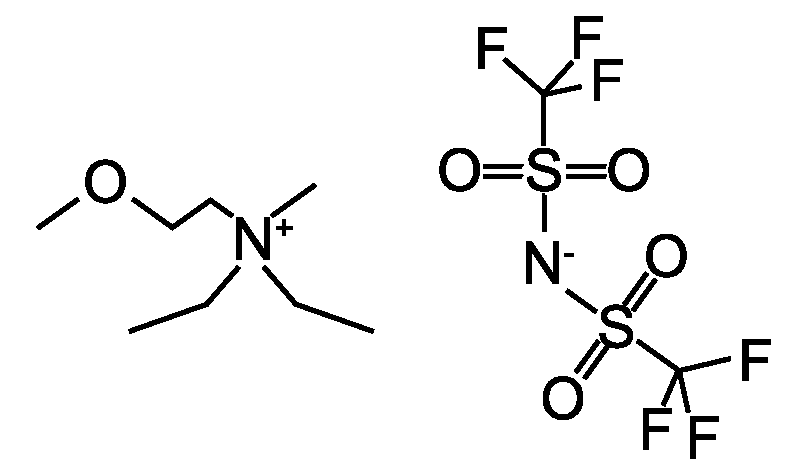
\includegraphics[width=100mm]{images/IL.eps}
\end{center}
 \caption{C$_{8}$H$_{20}$NO.C$_{2}$F$_{6}$NO$_{4}$S$_{2}$の構造式}
 \label{IL}
\end{figure}

かつてはイオン性液体や低融点溶融塩とも呼ばれたこともあるが,"ionic"をイオン性と訳す例が少ないことなどから今ではあまり使われていない.中でも室温において液体で存在できるものを特に室温イオン液体ということもあるが,一般にイオン液体というときは室温イオン液体を指すことが多い.\\


一般的な特徴として,上で述べたように電解質を加えずとも電流が流れ電位窓(有意義な電気化学測定が可能な領域)が広い.また蒸気圧が著しく低くほとんどゼロである.イオン伝導度は$10^{-5}\sim10^{-2}\,\mathrm{Scm^{-1}}$程度が報告されている.さらにイオン液体は耐熱性にも優れる.これらのユニークな性質から様々な分野に応用が期待されている.例えばその一つとして電解質としての利用である.その耐熱性も重なりイオン液体リチウムイオン電池がロケットに搭載されたこともある.その中でスピントロニクスで最もよく用いられる用途は電気二重層(electric doucle layer:EDL)を作成することによるキャリアドーピングである.イオン液体の電位窓の広さから固体ゲートより多くのキャリアドープが可能である点やデバイス作成に関して固体ゲートより簡便に使える点などがメリットとして挙げられる.そこでまずイオン液体による電気二重層の生成について述べたいと思う.その後に本研究で利用したイオン液体によるエッチング作用について述べる.

\subsection{イオン液体による電気二重層}
半導体だけでなくスピントロニクスデバイスにおいてもキャリアの制御はそれらの機能を発展させる重要な鍵になっている.キャリアドープは単なる伝導度を増大させる手段にとどまらず,高いキャリア蓄積は化学反応や相転移,磁気秩序の制御[Y. Yamada, K. Ueno, T. Fukumura, H.T. Yuan, H. Shimotani, Y. Iwasa, L. Gu, S. Tsukimoto, Y. Ikuhara, and M. Kawasaki, Science 332, 1065 (2011).,M. Weisheit, S. Fa ¨hler, A. Marty, Y. Souche, C. Poinsignon, and D. Givord, Science 315, 349 (2007).,K. Shimamura, D. Chiba, S. Ono, S. Fukami, N. Ishiwata, M. Kawaguchi, K. Kobayashi, and T. Ono, Appl. Phys. Lett. 100, 122402 (2012).],さらには超伝導状態の誘起など様々な現象を実現している.\\

長い間半導体であるシリコン(Si)とそれを自然酸化させた酸化シリコン(SiO$_{2}$)薄膜を核にして電界効果トランジスタ(field-effect transistors : FET)を作成するなど電界効果を用いる際は固体酸化物を利用した固体ゲートが主流であった.

しかしながら現在有機化合物やポリマー,複雑な酸化物などの今までの半導体と比較してキャリア数が低い物質がトランジスタの性能向上や今までにない新たな機能の開発において重要な役割を担うと考えられている[21 J. Veres, S. Ogier, G. Lloyd and D. Leeuw, Chem. Mater., 2004, 16, 4543–4555.22 A. Facchetti, M. H. Yoon and T. J. Marks, Adv. Mater., 2005, 17, 1705–1725.23 J. Robertson, Rep. Prog. Phys., 2006, 69, 327–396. ].このような様々な物質に対して十分なキャリアドーピングを行いたいと考えたときにゲート絶縁体が持つべき最も重要な特徴は一定以上のキャパシタンスである.キャパシタンスはゲート電圧を印可したときにどれだけの量のキャリアが誘起されるかを決める.以下ゲート電圧を印可する物質は半導体と考える.平行平板のキャパシタに蓄積した電荷$Q$は
\begin{eqnarray}
Q = CV
\label{eq:capaq}
\end{eqnarray}
と表せる.ただし$C$と$V$はそれぞれキャパシタンスと印可した電圧である.FETにおいてソース-ドレイン間を流れる電流$I_{D}^{SAT}$は飽和領域において
\begin{eqnarray}
I_{D}^{SAT} = \frac{\mu W C}{2L}(V_{G}-V_{G}^{th})^{2}
\label{eq:id}
\end{eqnarray}
と書ける.$L$,$W$はチャンネルの長さ及び幅を表し,$\mu$は移動度,$V_{G}$と$V_{G}^{th})^{2}$はゲート電圧とゲート電圧の閾値を表している.以上の式からわかるのは高いキャパシタンスを持つということは大きい電流が流れることや低いスイッチング電圧だけでなく高いキャリア濃度を誘起することを示している.\\
平行平板のキャパシタンスを思い出すと
\begin{eqnarray}
C = \frac{\epsilon_{0}\epsilon_{r}A}{d}
\label{eq:capa}
\end{eqnarray}
である.($\epsilon_{0}$と$\epsilon_{r}$はそれぞれ真空及び非誘電率,$A$は平行平板の面積,$d$は平板同士の距離である.)イオン液体の$\epsilon_{r}$の値はたかだか$1-10$程度であるがキャパシタンスは$\sim10\,\mathrm{\mu F\,cm^{-2}}$という大きな値を持つ.これはイオン液体が半導体との界面に電気二重層を形成する.電気二重層とは図\ref{EDL}のように半導体のホールとイオン液体のアニオン(陰イオンのこと.正に帯電した陽イオンはカチオンと呼ぶ.)がペアとなった部分のことであり,その結果半導体内にキャリア(ホール)をドープできる.
\begin{figure}[t]
 \begin{center}
  \includegraphics[width=100mm]{images/EDl.png}
\end{center}
 \caption{C$_{8}$H$_{20}$NO.C$_{2}$F$_{6}$NO$_{4}$S$_{2}$の構造式}
 \label{EDL}
\end{figure}

この電気二重層はSiO$_{2}$を用いた固体ゲートによるキャリアドープより何十倍もの効率が実現される[29].例えば例を挙げると厚さ$300\,\mathrm{nm}$のSiO$_{2}$を用いたゲートの持つキャパシタンスは$10\,\mathrm{nF\,\mathrm{cm^{-2}}}$なので,通常の非有機ゲートによる典型的なシートキャリア濃度は$10^{13}\,\mathrm{cm^{-2}}$程度である.この値は半導体の伝導率をある程度制御することは可能であるが,物質をキャリアドーピングによって超伝導状やフェロイック状態に相転移させるようなドラスティックな変化を誘起するには不十分と言わざるを得ない.しかしイオン液体による電気二重層を用いた方法は上記のような現象を発言させることが可能である.なぜならイオン液体によってドープさせるシートキャリア濃度は$10^{15}\,\mathrm{cm^{-2}}$という巨大な値を獲得できるからである.\\
次にイオン液体と固体との界面に形成される電気二重層について述べ,同時にそれのキャパシタンスについても考える.固体と液体との界面についての研究は数多くあり[38-40],それらの界面における電気化学的な振る舞いを説明する様々なモデルが存在する.ここではその中で特に有名な(a)Helmholtzモデル,(b)Gouy– Chapmanモデル(c)Gouy–Chapman–Sternsモデル,そして(d)Multilayerモデルの4つの違いをまとめる.\\


\begin{figure}[t]
 \begin{center}
  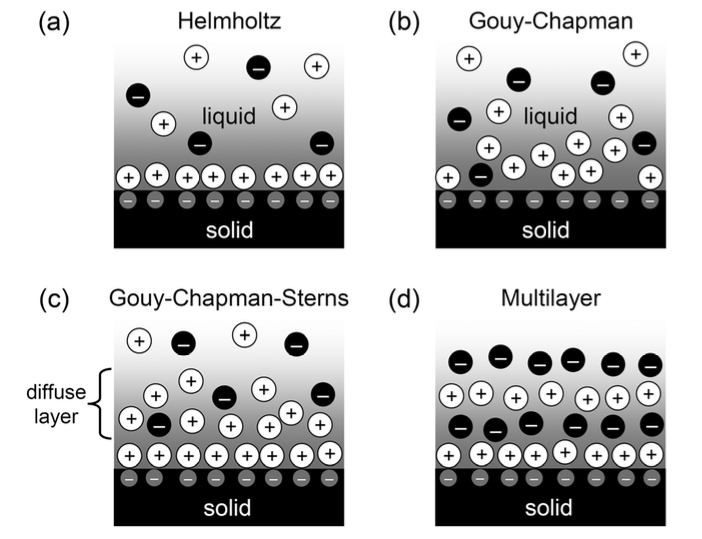
\includegraphics[width=100mm]{images/electrochemicalmodels.png}
\end{center}
 \caption{(a)Helmholtzモデル,(b)Gouy– Chapmanモデル(c)Gouy–Chapman–Sternsモデル,そして(d)Multilayerモデルによる固体/液体界面における電気化学的振る舞い.}
 \label{electrochemicalmodels}
\end{figure}


まず図\ref{electrochemicalmodels}(a)のHelmholtsモデルは液体中のイオンが一層だけ固体表面に層を形成し固体中の電荷を誘起すると考える[41].このモデルの利点は電気二重層のキャパシタンスの計算上の扱いが単純になるということである.そのため用いられるとも多い.一方図\ref{electrochemicalmodels}(b)のGouy– Chapmanモデルは電気二重層自体の拡散を導入している[42,43].\textcolor{blue}{これは固体表面から液体方向にポテンシャルがエクスポネンシャル的に減衰していくことを意味している.}しかしこのモデルだと大きい電気二重層を説明することができない.そこでこの問題を解決するためにGouy–Chapman–Sternsモデルが考案された(図\ref{electrochemicalmodels}(c)).Gouy–Chapman–SternsモデルはHelmholtsモデルとGouy– Chapmanモデルを組み合わせたモデルとなっている.つまり固体表面近傍のイオンが一層を形成しているHelmholtz層とイオンが拡散しているGouy–Chapman層を仮定することにより帯電量の高い電気二重層のキャパシタンスも説明できるようにしている.通常の電解質溶液の溶媒や溶質によるキャパシタンスの振る舞いはこのGouy– Chapmanモデルで十分に説明可能である.しかしながらこれらのモデルは元来希薄した電解質溶液の説明のために考案されたモデルであるため,Debye–Huckel理論[46]のように溶けているイオン同士はよく分離していて互いに相互作用はしないという仮定をおいている.これはイオン液体に関していうと完全に誤った仮定になってしまう.それは室温において溶媒を使わず溶かした"塩"からもよく分かる.そこで考えられたのが図\ref{electrochemicalmodels}(d)のようなMultilayerモデルである.これは融解した"塩"を説明するために確立された.このモデルは界面における空孔がBoltzmann分布に従うと仮定し,これによりイオンの層が多層に渡った構造中の歪みによって分極及びキャパシタンスが説明されている[47,48].このMultilayerモデルは他のモデルと比べて飛躍的によく実験結果を説明できるが,今のところ完全にイオンのみで形成された電解溶液の系を再現するようなモデルは確立されていない.\\

次に実際のイオン液体についての測定例についてまとめる.BaldelliらはBMIM-BF$_{4}$やBMIM-PF$_{6}$,BMIM-DCAなどのイミダゾール化合物(イミダゾール:C$_{3}$H$_{4}$N$_{2}$)をベースとしたイオン液体の表面構造についてマイクロ波(SFG:sum frequency generation)や電気化学インピーダンス(EIS:electrochemical impedance spectroscopy)を用いて研究し[49-52],BMIM-BF$_{4}$とBMIM-PF$_{6}$については隣接した金属との界面におけるイオンがHelmholtz-likeな振る舞いをしていて,そのポテンシャル降下は$3\sim 5\,\mathrm{\AA}$ ほどの範囲で起きていると結論づけている.さらにSFG測定の結果は"二重層"構造がポテンシャルに依存していることを示唆している.つまり\textcolor{blue}{(PZC:potential of zero charge)}が正のときはアニオンは金属表面に吸着しカチオンが持つイミダゾール環は表面に対して垂直に向いている.逆にPZCが負の時はカチオンが表面に対して平行に配向しておりアニオンは表面から離れているということが分かってる.このときの観測されたHelmholtz層の厚さはこの"二重層"を支持した結果になっていたが,アニオンの化学的性質のためBMIM-DCAについてはMultilayerモデルの方がより良く実験結果を再現していた.このときの一層の厚さはおおよそ$25\,\mathrm{\AA}$であった\\
Helmholtzモデルはイオン液体を電極と半導体間に挿入した場合のイオン液体/個体間における電気二重層と電極及び半導体とのポテンシャル差を予測できる.

\begin{figure}[t]
 \begin{center}
  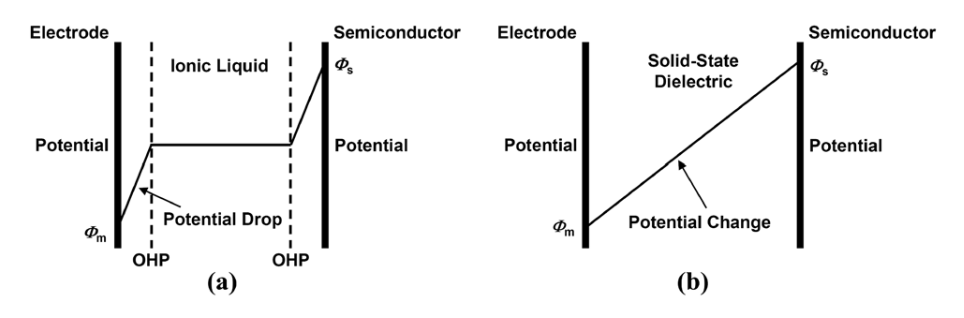
\includegraphics[width=100mm]{images/potentialchanges.png}
\end{center}
 \caption{半導体と電極に挟まれた誘電体((a)イオン液体,(b)固体絶縁体)におけるポテンシャル変化}
 \label{potentialchnages}
\end{figure}

イオン液体では図\ref{potentialchnages}(a)のようにポテンシャル降下はHelmholtz面の外側(OHP:outer Helmholtz plane)に限られる.このポテンシャル降下は電気二重層によるもので極めて薄い範囲で起き,これにより高いキャリア蓄積が半導体に誘起される.またこのOHPまでの距離は電解質の厚さ(イオン液体の種類)にほとんどよらない.この特徴は通常の固体絶縁体を用いたものとは全く異なっている.固体絶縁体中では図\ref{potentialchnages}(b)に示したようにポテンシャル降下は線形なため界面におけるキャリア蓄積は絶縁体の厚さに依存したものになる.


\subsection{イオン液体のキャパシタンス}
ゲート絶縁体のキャパシタンスはそれ自体の性能を判断するときの重要なパラメータである.FujimotoらはEME-TFSIとDEME-BF$_{4}$,BMIM- TFSI,BMIM-BF$_{4}$,BMIM-OTf,BMIM-PF$_{6}$の6つのイオン液体について$10^{-1}\sim10^{5}\,\mathrm{Hz}$の範囲でキャパシタンスの周波数依存性を測定している[53].

\begin{figure}[t]
 \begin{center}
  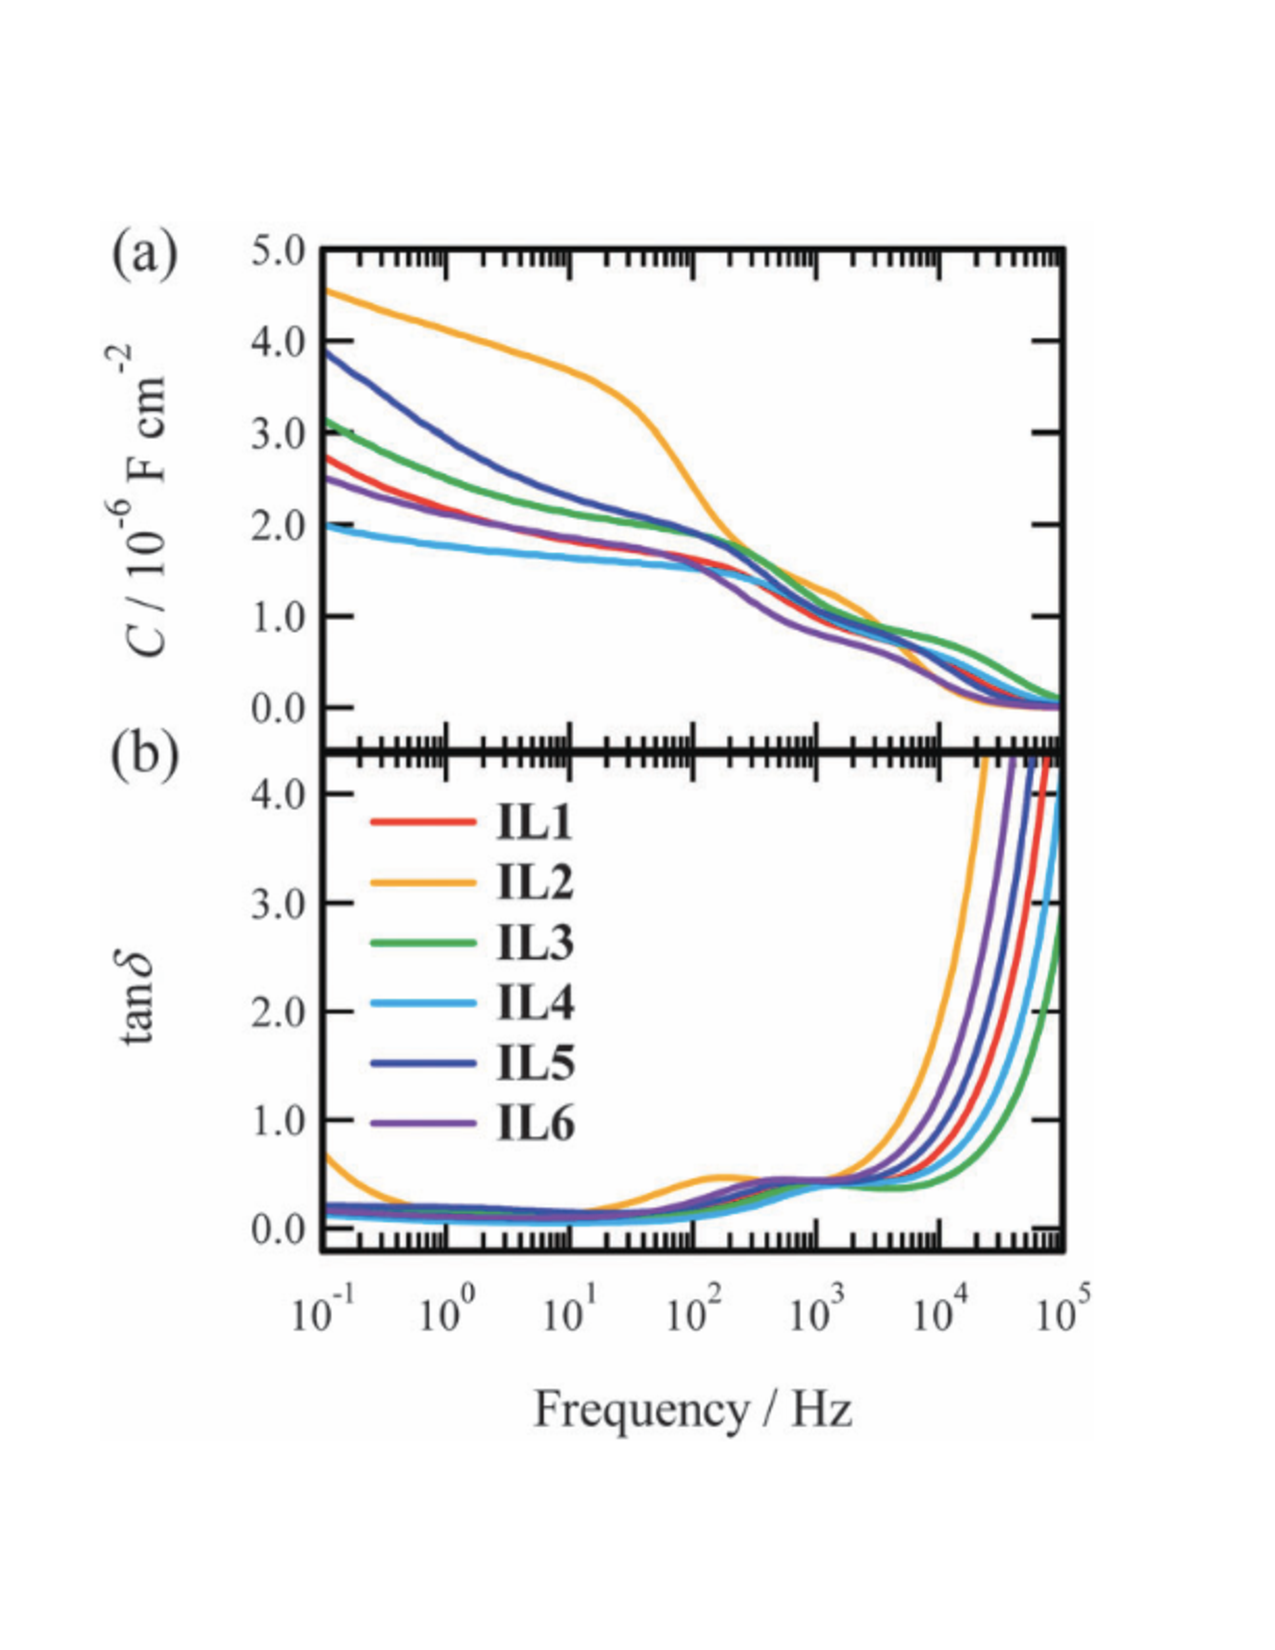
\includegraphics[width=100mm]{images/ILcapacitance.pdf}
\end{center}
 \caption{(a)キャパシタンス及び(b)tan$\delta$の周波数依存性.IL1: DEME-TFSI,IL2:DEME-BF$_{4}$,IL3:BMIM-TFSI,IL4:BMIM-BF$_{4}$,IL5:BMIM-OTf,IL6:BMIM-PF$_{6}$.}
 \label{ILcapacitance}
\end{figure}

その結果が図\ref{ILcapacitance}(a)である.$10^{2}\,\mathrm{Hz}$以下の低い周波数領域ではイオン液体のキャパシタンス$C_{\mathrm{IL}}$の値が$10^{-6}\,\mathrm{F\,cm^{2}}$以上ととても大きく,またイオン液体によって値が大きく異なっている.一方$10^{2}\,\mathrm{Hz}$以上の範囲ではイオン液体の種類によらず同じように減少している.図\ref{ILcapacitance}(b)は損失係数tan$\delta$の周波数依存性を示している.

\begin{figure}[t]
 \begin{center}
  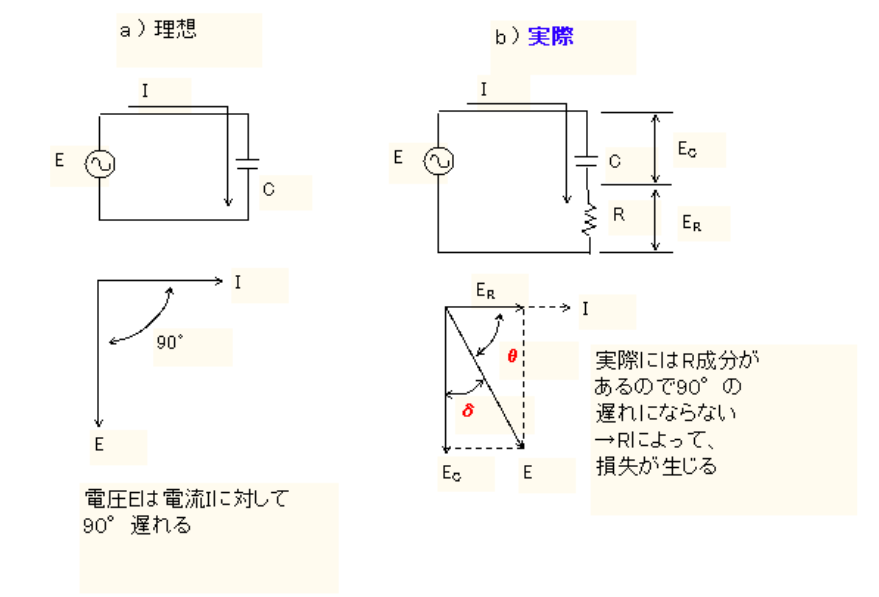
\includegraphics[width=100mm]{images/tandel.png}
\end{center}
 \caption{コンデンサの理想と実際}
 \label{tandel}
\end{figure}

損失係数とはキャパシタンスがどれだけ抵抗成分を含んでいるかを示している値である.図\ref{tandel}のようにキャパシタンス測定において理論的には電圧は電流に対して$90^{\circ}$遅れるはずであるが,実際には回路中の抵抗によってこの位相差が$90^{\circ}$からズレる.このズレの角度を$\delta$とすると損失係数$D$及び品質係数$Q$は

\begin{eqnarray}
\tan\delta = \frac{1}{Q} = D
\label{eq:tandel}
\end{eqnarray}

となる.図\ref{ILcapacitance}(b)を見ると損失係数は$10^{2}\,\mathrm{Hz}$以下で小さく,周波数を増加していくと大きくなっている.また損失係数は以下の式でも表せる.


\begin{eqnarray}
\tan\delta = \frac{I_{\mathrm{R}}}{I_{\mathrm{C}} }= \frac{1}{\omega C_{\mathrm{IL}}R_{\mathrm{P}}}
\label{eq:tandel2}
\end{eqnarray}

ここで$R_{\mathrm{P}}$は並列抵抗及び$\omega$は角運動量周波数であり$I_{\mathrm{R}}$と$I_{\mathrm{C}}$はそれぞれ$C_{\mathrm{IL}}t$と$R_{\mathrm{P}}$に流れる電流である.$R_{\mathrm{P}}$の周波数依存性は線形なので図\ref{ILcapacitance}(b)における$10^{2}\,\mathrm{Hz}$より大きい周波数における損失係数の増大は$C_{\mathrm{IL}}$の低下によるものだと推測できる.このキャパシンタンス及び損失係数の周波数依存性はイオン液体の電気二重層は低い周波数において効果的に現れることを示している.加えてこれらの高い周波数における振る舞いはイオン液体のアニオン及びカチオンが電極界面における空間的に配列しており,その形成が$10^{2}\,\mathrm{Hz}$以上の周波数に対してほとんど追従できていないことを示している.ここからイオン液体は電気二重層が形成がゲート電圧の周波数に追従していると考えられる$10^{2}\,\mathrm{Hz}$以下の周波数において$10^{^6}\,\mathrm{Fcm^{-2}}$という巨大なキャパシタンスを実現し,$10^{15}\,\mathrm{cm^{-2}}$という大きなキャリア蓄積を誘起できるとわかる.これらは通常の固体ゲートと比較して極めて大きな値である.




以上はイオン液体による電気二重層キャパシンタンスを用いることによって固体ゲートに比べ大きな電界効果を与え,効率的かつ簡単にデバイスのキャリア制御を行う方法を述べた.しかし本研究ではこの電解効果を与える作用を用いず,この効果を与えるに有効な電場以上の電場をイオン液体に与えることによって電気分解反応を誘起し接した金属をエッチングする方法のアイデアについて述べたいと思う.

\subsection{イオン液体による電気化学エッチング}


\section{グラフェン}\label{sec:graphene}
グラフェンが物性物理学において注目される物質となり既に10年以上が過ぎている.2005年頃のGeimらのグループ、およひびKimらのグループによるグラフェンの合成及び特異な量子ホール効果の発見[1, 3]によりグラフェンの研究の人気は始まった.現在ではグラフェンの基礎的な研究はほとんどされていると言われているがその応用などの研究を含めれば今でもホットな研究テーマであると言える.この章ではなぜ本研究でグラフェン用いたのかという理由を明白にするため,グラフェンの持つ物理的性質における普遍的な特徴をまとめグラフェンがどれだけ興味深い材料なのかを述べる.そしてスピントロニクスにおけるグラフェンの位置を述べ,これからのグラフェン研究の発展において必要な研究を明らかにし本研究の重要性を述べたい.また本研究で用いたグラフェンは一層のグラフェンであるがグラフェンを数層重ねたグラフェンも同様にグラフェンと呼称する.ここでは誤解を避けるため以下では単層のグラフェンをグラフェンといい,層に言及しない限り単層グラフェン(SLG:single layer graphene)をグラフェンということにする.

\subsection{グラフェンの作成方法}\label{subsec:graphene}
まずグラフェンの作成方法について述べる.グラフェンの作成方法にはいくつか候補がある.代表的なものはFig.\ref{fig:graphene_howtomake}にまとめた.

\begin{figure}[t]
 \begin{center}
  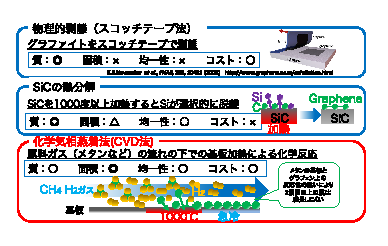
\includegraphics[width=120mm]{images/graphene_howtomake.eps}
  \end{center}
   \caption{グラフェンの代表的な作成方法.}
 \label{fig:graphene_howtomake}
\end{figure}


一つは初めてグラフェンの作成に成功したスコッチテープである.この方法はグラファイトの試料をスコッチテープを用いて剥離を繰り返すことで炭素の層を薄くしていきグラフェンを作成し基板に圧着する.この方法で作成したグラフェンは高品質であることが知られ,最大の移動度を測定されたものもスコッチテープ法で作られた.しかしスコッチテープで剥離を繰り返すため,手に入る試料のサイズは小さく加工も難しい.
SiCの熱分解を用いた方法はその名の通りSiC基盤を1000$\rm\ C^{\circ}$で加熱することにより表面にグラフェンが成長させる方法である.SiCを高温で加熱すると表面においてSiだけが選択的に脱離する.すると表面に残った炭素原子同士が自発的に結合しグラフェンを成長する.この方法によるグラフェンも質が良いことで知られる.しかし大面積のグラフェンを得られてもグラフェンの総数が制御しにくいことやコスト面が高価なためこの方法を選択しなかった.
化学気相蒸着,もしくは化学蒸着(CVD:Chemical Vipor Deposition)法は原料のガス(ここではエタノールガス)を流した中で基板を加熱することで基板表面で化学反応が起きグラフェンが成長する方法である.この方法は他の作成方法に比べグラフェンの質は劣るがコストが低く,基板の選択肢の多さや加工のしやすい.本研究ではこのCVD法を用いてグラフェンを作成した.

\subsection{二次元電子系としてのグラフェン}
この章ではグラフェンの特異な電子状態を述べるために,まずグラフェンの結晶性を物理化学的な構造からまとめる.
グラフェンはFig.\ref{fig:graphene}ベンゼン環が平面状に連なった二次元物質と呼ばれる材料であり,炭素原子がsp$^{2}$混成軌道によりハニカム構造をなしている.
\begin{figure}[t]
 \begin{center}
  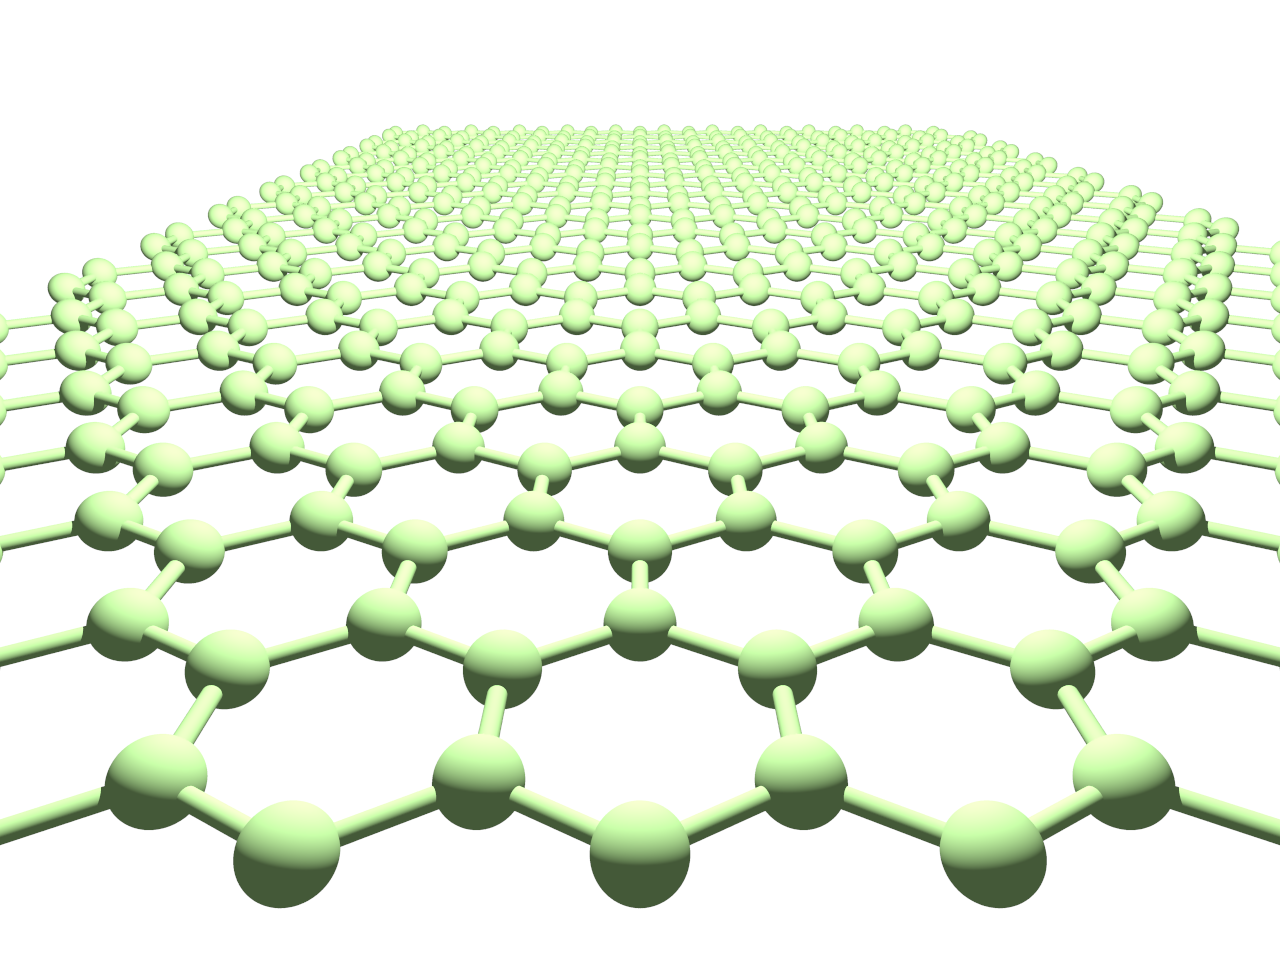
\includegraphics[width=90mm]{images/graphene.png}
  \end{center}
   \caption{グラフェンの概略図.炭素原子がハニカム構造を保って二次元平面状に連なっている.}
 \label{fig:graphene}
\end{figure}

この炭素は強固な共有結合を持つということで有名であり,実際にsp$^{1}$,sp$^{2}$,sp$^{3}$混成軌道という様々な結合状態をもつことを反映し,一次元物質のポリアセチレン,二次元物質のグラフェン,三次元物質のダイアモンドという形態が存在する.(シリコンも炭素と同族であり同じような形態を持つが,自然界に存在するという点では炭素特有である.)
理論的考察からはグラフェンのような二次元物質(しかも十分マクロなサイズで)が合成できるという事実は驚くべきことである.PeierlsやLandau,Merminらが示したように,低次元物質は長波長のエネルギー揺らぎに対して不安定であり,理論的には純粋な一次元や二次元の物質は存在できないと予想されていた[11].しかしこの予想に反してグラフェンは十分大きな面積において二次元構造を維持していると考えられている.このような理論的には存在できない物質が実際に存在できてしまうということが自然科学の面白いと思える部分であり,実験家の存在意義の一つのように感じる.ただしこのストーリーには続きがある.
\begin{figure}[t]
 \begin{center}
  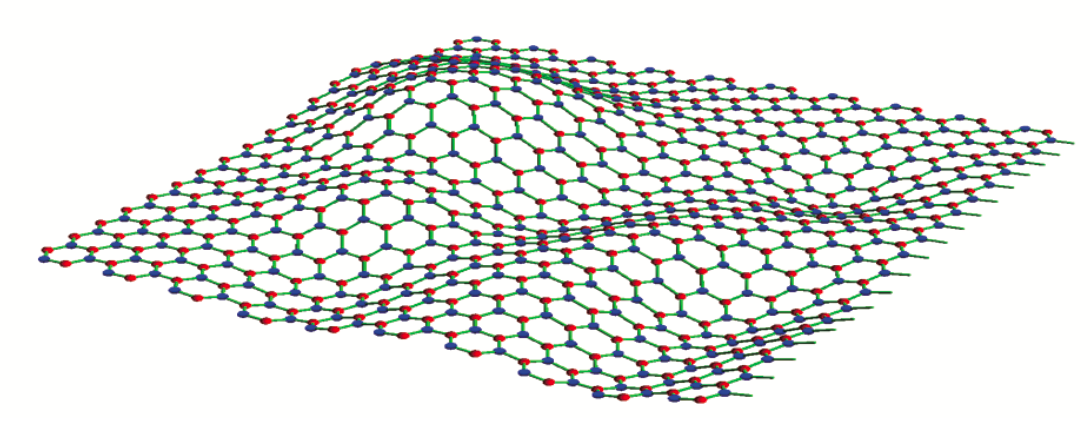
\includegraphics[width=100mm]{images/ripple.png}
  \end{center}
   \caption{グラフェンにおけるリップル構造.これが存在するために二次元構造を保ったまま存在することができると考えられる.}
 \label{fig:ripple}
\end{figure}

実際に存在しているグラフェンを観察すると完全な二次元平面ではなく,Fig.\ref{fig:ripple}のような三次元的な凹凸(リップル:ripple)を持った構造になっており,この長波長のうねりがグラフェンにおいて重要な役割を担っていると考えられている.
つまり二次元物質であっても存在しているのは三次元空間であり自由度も三次元方向に許される.この自由度がゆらぎにおけるエントロピーを吸収し,安定な二次元構造を保っているという考察である.リップルが大きすぎるとsp$^{2}$結合が歪みグラフェン全体の電子系のエネルギー的に損をするため,局所ごとに変形を小さくしそのエネルギー損失を抑えつつ適度なリップルが存在することによりエントロピーを解放するというシナリオのもと,リップルを持った二次元物質が存在できると考えられる.


\subsection{グラフェン中のディラック電子}

次にグラフェンの電子系についてまとめる.
グラフェンの合成は2000年初頭に成功しそこから実際にグラフェンを用いた実験が爆発的に行われたが,理論的には1940年代ごろから考案されておりその特異な電子状態を最初に指摘したのがWallaceである[5].一般的に物質の電子状態は半導体を含む絶縁体と金属に大別される.絶縁体は結晶の周期性による量子力学的干渉効果に起源を持つバンドギャップ構造で特徴付けられ,金属はフェルミ面及びそれをまたぐ電子と正孔の対生成によるギャップレス励起を持つことが知られている.さらに半貴族というカテゴリーがあり,これは通常半導体のギャップレス状態を指す.ギャップレスという意味ではグラフェンも半金属(実際にグラフェンを面直方向に積層したグラファイトは電子及び正孔ポケットを持つ半金属である.)である.しかしグラフェンが特異な点はフェルミエネルギーを貫くバンド分散の傾きがゼロではない(フェルミ速度が有限)点である.これはグラフェンが通常のフェルミエネルギーのバンドの端において電子の速度がゼロになるという常識と反した特異な半金属であるということを示している.この特徴はグラフェンがハニカム構造を持つことに起因する.ハニカム構造はFig.\ref{fig:graphene_vector}のように単位胞中に対称性の異なるに原子を持つ.(図では原子の白と黒で分けている.)

\begin{figure}[t]
 \begin{center}
  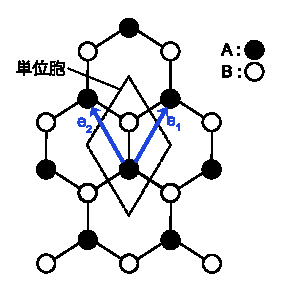
\includegraphics[width=80mm]{images/graphene_vector.eps}
  \end{center}
   \caption{グラフェンのハニカム構造の概要図.点線の範囲が単位胞を表し,対称性の異なる炭素原子サイトを黒円と白円で分けてそれぞれA,Bと表した.$e_{i},i=1,2$は基本並進ベクトルである.}
 \label{fig:graphene_vector}
\end{figure}

この格子はsp$^{2}$混成軌道が互いに$120\ ^{\circ}$異なる三方向に結合していて,化学ではこれを\sigma 結合という.炭素の持つ最外殻電子は4つであり,残りの一つは格子面($x,y$)の垂直方向に伸びたp$_{z}$軌道に入る.この電子が原子間を移動し,この結合を\pi 結合と呼び,この電子によるバンドを\pi バンドと呼ぶ.
実際にグラフェンの電気的性質を担っているのはこの\pi バンドで,フェルミエネルギーもこの\pi バンドを横切っている.これは普通tight-bindingモデルで扱う.このときのハミルトニアンは

\begin{eqnarray}
\mathcal{H} = t\sum_{x}[c_{B}^{\dag}(x)c_{A}(x) + c_{A}^{\dag}(x+e_{1})c_{B}(x) + c_{A}^{\dag}(x+e_{1})c_{B}(x)]
\label{eq:tight-binding}
\end{eqnarray}

のようにかける.ここで$c_{i}^{\dag}$は$i=\rm A$または$\rm B$に電子を生成する生成演算子,$t$は最近接原子への飛び移り積分である.グラフェンにおける実際の値は$t \simeq -3\rm\ eV$である.ハミルトニアンを波数表示するために$c_{i}(x)=\sum_{k}e^{ikx}c_{i}(k)$のようにブロッホ形式に書き直すと

\begin{eqnarray}
\mathcal{H} = \sum_{k}\textbf{\textsl{c}}^{\dag}(k)H(k)\textbf{\textsl{c}}(k),\\
H(k) = 
\begin{pmatrix}
0 & D(k) \\ 
D^{*}(k) & 0  
\end{pmatrix}
\label{eq:tight-binding2}
\end{eqnarray}

となる.ここで$\textbf{\textsl{c}}^{\dag}\equiv(c_{\rm B}^{\dag}(k),c_{\rm A}^{\dag}(k))$,$D(k)=t(1 + e^{\ik_{1}}+e^{\ik_{2}})$である.各$k$ごとに対角化すると永年方程式が$\epsilon^{2}(k)=|D(k)|^{2}$であることからエネルギー分散は$\epsilon(k)=\pm|D(k)|$となることが分かる.またグラフェンのバンド分散はFigのようになり,波数空間の2点($K$点と$K'$点)でエネルギーギャップが線形に交差する.この形をディラックコーンと呼ぶ.この交差してギャップが閉じた点をディラックポイントといい,この点付近の分散関係が質量ゼロのディラック粒子と形式的に類似しているためグラフェン中の電子は相対論的だと表現される.
グラフェンにスピン軌道相互作用があるときディラックコーンのギャップが開く.炭素は軽い原子のためスピン軌道相互作用は弱く,炭素イオンのスピン軌道相互作用による分裂は$7.86\rm\ meV$である.[Kramida, A., Ralchenko, Y., Reader, J. & Team, N. A. NIST Atomic Spectra Database (version 5.1) http://physics.nist.gov/asd (National Institute of Standards and Technology, 2013).]そのため当然グラフェンの内因的なスピン軌道相互作用は小さい.グラフェンのスピン軌道相互作用はバンド状態に強く依存しているため,他原子のドープやゲーティング,基板などの外因的な効果もよく反映する.グラフェンにおけるスピン軌道相互作用の小ささはスピン流の注入や制御の困難さを表すため,グラフェンのスピン軌道相互作用を増大させる方法は注目された研究テーマである.

\subsecton{グラフェンにおける光吸収}
次にグラフェンと光関係についてまとめる.本研究においてグラフェンの評価に用いた測定にラマン分光測定がある.ラマン分光は光の非弾性散乱であり,グラフェンの状態によって光との相互作用が変化するためこれによりグラフェンの評価が可能となる.その基礎としてグラフェンのバンドと光吸収について述べる.

グラフェンは可視光や赤外光などの長波長の光を吸収し赤外光を発光する.このような光吸収と発光に関わっているのがグラフェンにおける\pi バンドである.(価電子帯のバンドを\pi バンド,伝導帯を$\rm\pi^{*}$バンドと呼び分けることもある.)\pi 及び$\rm\pi^{*}$バンドのエネルギーバンドは、ハニカム構造のブリルアン領域の角であるK点,つまりディラックポイントで接する。電子は\pi バンドのみを占有するためフェルミエネルギーはディラックポイントでのエネルギーになる。グラフェンにゲート電圧を加えて電荷を注入した場合には、フェルミエネルギーはこのディラックポイントからずれる。可視光や赤外光などの吸収は\pi バンドから$\rm\pi^{*}$バンドへの遷移によって起こる.可視光より大きなエネルギーを持つ光に対しては、\sigma バンドから$\rm\sigma^{*}$バンドへの遷移や1s軌道から\sigma バンドや$\rm\sigma^{*}$バンドへの遷移によって起こることもある.
光の吸収強度は光の振動する電場ベクトル$E$と原子のもつ遷移双極子モーメントベクトル$D$との内積で与えられる.ここで遷移双極子モーメントとは,光の電場によって原子のまわりの電子分布が変位し負の電荷が誘起され,原子核の正の電荷とともに定義される双極子モーメントのことである・遷移双極子モーメントは光の電場の振動数と同じ振動数で振動するがここで振動の位相が少し遅れる.位相が少し遅れると光が電子に対して仕事をするので光のエネルギーが電子に与えられる.これが光吸収の原理である.光吸収スペクトルの強度は,この遷移双極子モーメントの大きさを入射光のエネルギーの関数として求めることで理論的に計算できる.実験的には光吸収スペクトルを測定することで得られる.上記のようにグラフェンにおける可視光吸収は\pi バンドから$\rm\pi^{*}$バンドへの励起によるが,このときグラフェン1層あたり$2.3 \%$の光が吸収されることが知られている.この吸収強度はグラフェンの層数に比例しているため,光学顕微鏡の元でグラフェンの層数が濃淡で現れる.グラフェン一層の厚さは$0.335\rm\ nm$であるため,グラフェンの光の吸収強度が大きいことがわかる.
光によって励起された電子および価電子帯に発生した正孔がキャリアになり光電流が流れる.光電流とは光を当てた時だけ流れる電流のことを指す.光を当てていない状態で試料に流れる電流を暗電流という.光が当たっていなくても有限温度では電子はフェルミ分布に従って熱的に励起しているので電子とホールを持ち電流を流すことができる.グラフェンでは\pi バンドと$\rm\pi^{*}$バンドは1点で接するのでディラックポイントでの電子の状態密度は0であり電流を担うキャリアの数は少ない.にもかかわらずグラフェンがよく電気を流すのは一つ一つの電荷の移動度の値が非常に大きいからである.電流の大きさは単位体積当たりの電荷の数,一つの電荷の平均速度,電流の流れる断面積の大きさの積で与えられる.一つの電荷の速度は電場と移動度の積で与えられ,移動度は電荷が自由に加速できる時間(緩和時間)に比例し,電荷の質量に反比例する.グラフェンの移動度が大きい理由はディラックポイント付近の電子やホールのエネルギー分散が波数$k$に比例しキャリアーの有効質量がゼロになるからである.有効質量がゼロになるのは相対論的なエネルギーの式$E = \sqrt{m^{2}c^{4} + p^{2}c^{2}}$において$m=0$とおくと$E$が$p=\hbar k$に比例することに対応している.電子のエネルギー$E$が $k$に比例することは非常に特殊な状況である.たとえば電子の群速度は電子のエネルギーによらず一定である.グラフェンの場合には群速度は$106\rm\ m/s$ であり光速の300分の1にもなる.欠陥やフォノンなどで電子が散乱されて運動量の向きが変わっても速度の大きさが変わることはない.フォノンなどの非弾性散乱の場合には,運動量の向きやエネルギーの値は散乱後で変化するが速度は変化しない.特に散乱が無いような結晶性の高い試料でかつフォノンが発生しにくい低温の場合には,移動度は$1\times10^{6}\rm\ cm^{2}/Vs$という驚異的に高い値を示す.したがってTHz領域の高い振動数でも動作可能な素子が作ることができ ることが期待されている.実際にグラフェンで作られたFET(電界効果トランジスター)は$500\rm\ GHz$の遮断周波数(追従できる最高の周波数)が観測されている.

\section{本研究の目的}
本研究の目的はST-FMR測定を用いてDamping-likeトルク及びField-likeトルクを定量する際に単一の試料を用いて膜厚依存性を測定するために,イオン液体の電気化学反応によって強磁性金属をエッチングしながら同時にST-FMR測定を行いトルク定量を実現することである.この研究目的を達成することにより同一試料を作成するのが困難な物質の膜厚依存性や測定とエッチングを同時に行うことが可能になる.つまりこの研究が達成されることによりスピントロニクス分野に限らず材料研究全ての分野の研究進度を加速させることができる.

\section{本論文の構成}
本論文の構成は以下のようになっている.まず第2章で本研究において行った資料作成および実験方法,スピン軌道トルクの定量の仕方について述べる.そして第3章では実際に行った測定について述べ,その結果を説明し考察する.




